\documentclass[12pt]{article}

\usepackage{graphicx}
\usepackage{svg}
\usepackage[
    backend=biber,
    style=authoryear,
    sorting=nyt
]{biblatex}
\addbibresource{bibliography.bib}

\newcommand{\code}[1]{\texttt{#1}}

\usepackage[utf8]{inputenc}
\usepackage[
    twoside,
    top=1in,
    bottom=0.75in,
    inner=0.5in,
    outer=0.5in
]{geometry}

\usepackage{tcolorbox}
\tcbuselibrary{skins}
\usepackage{minted}
\usepackage{color}
\usepackage{tikz}
\usetikzlibrary{calc}
\usepackage{tabularx,colortbl}
\usepackage{amsfonts,amsmath,amssymb}
\usepackage{titling}
\usepackage{mathrsfs}
\usepackage{calc}
\usepackage{graphicx}
\usepackage{svg}
\usepackage[
    backend=biber,
    style=authoryear,
    sorting=nyt
]{biblatex}

\addbibresource{bibliography.bib}


\title{Modelling weather and the climate}
\author{Heather Tweedie}
\date{March 2023}

\linespread{1.25}

\begin{document}

%%%% Format Running Header %%%%%
\markboth{\theauthor}{\thetitle}

%%%% Insert the Title Information %%%
\maketitle

\section{Introduction}

    The threats posed by climate change brought about primarily by increases in anthropogenic emissions means it is necessary 
    to develop models that are capable of predicting the impacts of these changes. The models used to predict long-term future 
    climate variations are similar to those used to model present weather and climate conditions (\cite{raisanen_2007_how}), 
    and as such, it is important that these models are well-understood.
    
    This study aims to determine if the weather and climate at a location can be predicted using basic machine learning techniques. 
    Two main research questions are proposed:
    
    \begin{enumerate}
      \item How accurately can a model predict the climate of a location a year in advance?
      \item Can a model predict the weather at a location any better than assuming the weather tomorrow will be the same as the 
      weather today?
    \end{enumerate}

    These questions are investigated by training two neural networks on daily weather observations, and testing these models to 
    determine the accuracy with which they can predict future weather and climate variables.
    
\section{Data used}

    The data used in this study were obtained from the Global Historical Climate Network (GHCN). GHCN-Daily (GHCND) (\cite{menne_2012_global}) 
    is a database of daily weather summaries featuring data from over 80,000 stations in 180 countries (\cite{menne_2012_an}). Approximately 
    two thirds of the stations report precipitation data only, however many stations report maximum and minimum temperatures, snowfall and 
    depth in addition. The data come from a number of global sources including the National Oceanic and Atmospheric Administration, the 
    European Climate Assessment and Dataset, and the South African Weather Service, and are subjected to automated, unsupervised quality 
    assurance tests.
    
    Only stations which are part of the GCOS Surface Network (GSN) were included in this study. As of March 2019, 1023 stations were part 
    of this network (\cite{oakley_2019_gcos}), providing an approximately uniform coverage of the globe with high-quality data of a good 
    length (\cite{theglobalclimateobservingsystem_gcos}) (Figure 1).

    \begin{figure}
        \centering
        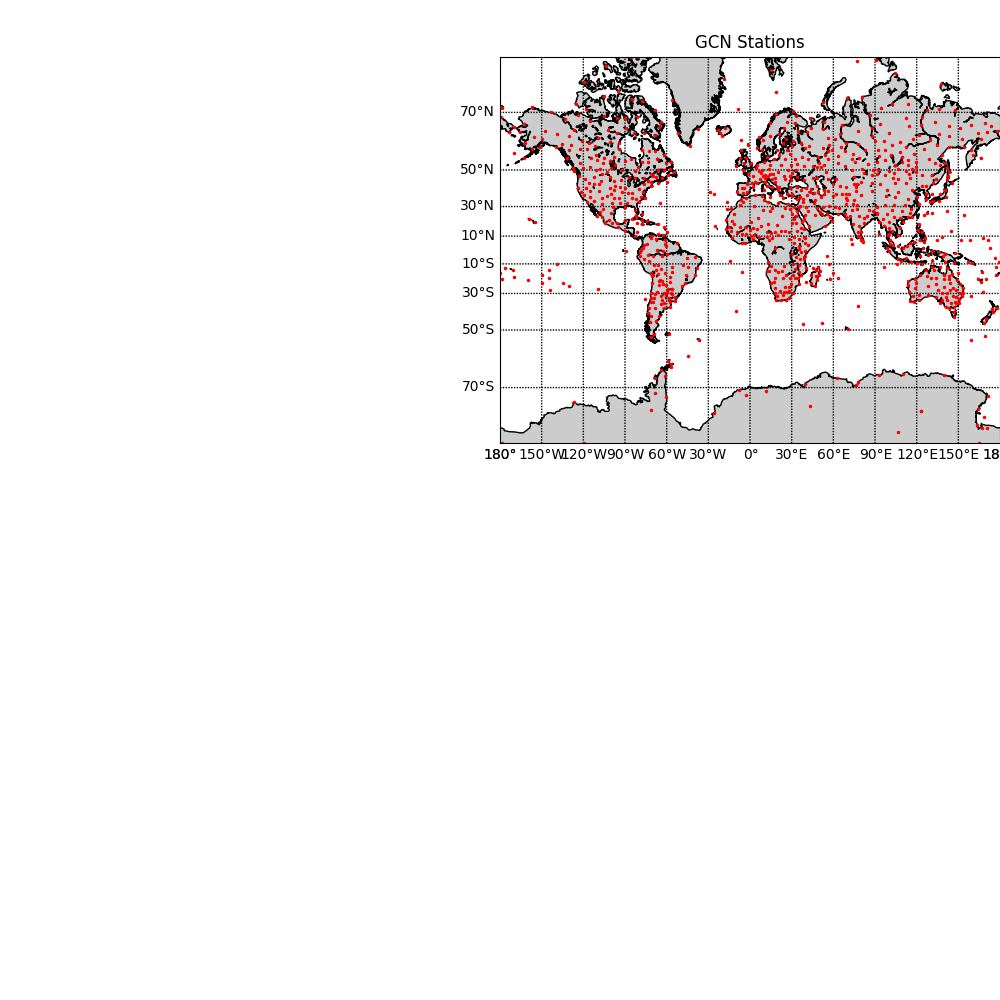
\includegraphics[scale = 1.0]{all_stations.png}
        \caption{All stations included in the GCOS Surface Network (GSN). Stations are marked as red points and plotted on a basemap of 
        the Mercator projection. The network provides a relatively uniform coverage of global land areas.}
        \label{fig:all_stations}
    \end{figure}

    To study the first research question, regarding climate prediction, the focus was put on the prediction of maximum temperature values 
    at the station ASN00003003, located at Broome Airport, Australia. The second research question is investigated using maximum temperature 
    and precipitation data from station ASN00030124, located at Georgetown Airport, Australia.

\section{Predicting the weather}

    \subsection{Methodology}

    To filter the stations used, the number of missing data points from the temperature and precipitation data were counted; the stations 
    with no or fewer than 100 gaps were focused upon for study. A station to investigate was selected on this basis, and the data for that 
    station acquired from a course-provided directory of GSN station data files. In this case, station ASN00003003, located at Broome 
    Airport, Australia, was selected, for it's quality of data and convenient length. Time-series data for the specified variables were 
    then extracted from this station's data file and stored in separate instances of the `Variable` class with fields for the values and
    their corresponding dates. These dates were then converted from their original ‘DateTime’ format, to the number of days since the first 
    observation, in order to ease plotting later.
    
    At this point, the data were normalised, bringing them all to a similar scale to improve the performance and stability of the model 
    during training. This was carried out by subtracting the mean of the entire dataset from each value, then dividing by the maximum 
    value found in that set. Figure 2 shows the maximum temperature and precipitation data extracted from this station's file.
    
    Following normalisation, the data were concatenated from individual 1-d arrays into a single n-d array, then subdivided into training, 
    validation and testing datasets. There were a number of considerations to make when deciding on ratios for these datasets. The training 
    dataset must be sufficiently large to prevent high variance during training of the model, but the validation and testing datasets must 
    be large enough to prevent high variance when evaluating the model. The validation dataset is used to tune the hyperparameters of the 
    model, and given that in this case there are relatively few of these, a smaller validation dataset is used. A final training to testing 
    to validation ratio of 0.7 : 0.2 : 0.1 was used.
    
    The divided datasets were then split into a series of overlapping windows, with lengths equal to a defined window size, and an associated 
    value a number of data points ahead in the time series, dictated by a defined offset. These are the input windows and targets on which 
    the model will be trained, validated and tested. The window size dictates how much data the model is trained on in a single batch. If 
    this is too small, the model will not perform well, however it must be smaller than the size of the validation dataset minus the offset, 
    otherwise it will be impossible to shape the dataset as necessary in later steps. It was found during testing that a window size of 60 
    worked well and gave a good performance. An offset of 1 was used, meaning the model predicts one day ahead. These windows are reshaped 
    from (number of windows, window size) to (number of windows, window size, number of features), where ‘number of features’ is the number 
    of variables being used in this model’s training, in this case, two.
    
    The model to be trained on the input data described above employs layers of long short-term memory, as described by Hochreiter and 
    Schmidhuber (\cite{hochreiter_1997_long}). This layer type has the advantage of allowing the model to 'remember' a sequence of values 
    and predict on the basis of these, rather than a more limited number as in the case of a dense layer. The table below describes the 
    structure of the model used.
    
    \begin{table}[H]
    \centering
        \begin{tabular}{ |p{2.5cm}|p{4cm}|p{3.5cm}|p{4cm}| }
         \hline
         Layer Type & Output Shape & No. of Params & Activation Function \\
         \hline
         LSTM  & (None, None, 64) &  17152 & relu   \\
         LSTM  & (None, 128)      &  98816 & relu   \\
         Dense & (None, 2)        &  258   & linear \\
         \hline
        \end{tabular}
    \end{table}

    As only two variables were predicted using this model, the complexity was kept relatively low to reduce run-time and to avoid over-fitting 
    the data. During testing it was found that using the linear activation function with the LSTM layers kept the predictions relatively 'flat' 
    and prevented them from accurately modelling the height of peaks and troughs in the data. The relu (Rectified Linear Unit) activation 
    function did not have this effect, so this was used for those layers. 

    The model was trained over fifty epochs, at which point the training and validation losses had approximately levelled, and predictions could 
    be made using the trained model and testing input dataset. The data were then de-normalised in order to plot them as absolute values.
    
    \begin{figure}
        \centering
        \includesvg[scale = 0.75]{weather_input_data.svg}
        \caption{Maximum daily temperature and daily precipitation data used for training, validating and testing the model. Top: maximum daily 
        temperature in degrees Celcius. Bottom: daily precipitation in mm.}
        \label{fig:weather_input_data}
    \end{figure}

    
    \subsection{Results}

    The loss achieved by the model during training is shown in Figure 3. The loss drops rapidly in the first five training epochs, then 
    decreases gradually, reaching a minimum of 0.0018 at the final epoch. The validation loss is much lower than this, however; it follows 
    a similar path, dropping rapidly at the beginning of training, but levels out at approximately 0.00095 by the tenth training epoch.
    
    \begin{figure}
        \centering
        \includesvg{weather_loss.svg}
        \caption{Loss of the model during training. Blue line: loss achieved during training. Orange line: loss achieved when validating the model.}
        \label{fig:weather_loss}
    \end{figure}

    Figure 4 shows both the observed values and those predicted by the model for the maximum temperature and the precipitation over the 
    target period. Overall, both the temperature and the precipitation predictions seem to model the general shape of the observations 
    well. The temperature seems to follow an approximately sinusoidal annual cycle, with peaks and troughs roughly six months apart from 
    each other. The precipitation data also shows higher precipitation during the times with greater temperatures. The predicted precipitation 
    data, however, features greater variability during the periods of low to no observed precipitation.
    
    \begin{figure}
        \centering
        \includesvg[scale = 0.7]{weather_prediction.svg}
        \caption{Observed and predicted values for maximum temperature and precipitation. Blue lines show data predicted by the model; orange 
        lines show observed data.}
        \label{fig:weather_prediction}
    \end{figure}

    Figure 5 shows the observed and predicted temperature and precipitation data in greater detail, limiting it to the first six months of 
    data. The values for the assumption that tomorrow's weather will be the same as today's are also plotted. The temperature observations 
    and predictions appear to match closely, especially when considering the overall trends. The temperatures predicted by the model do however 
    appear to frequently cut peaks and troughs by a small amount. The precipitations predicted by the model are less accurate however, with 
    the peaks cut substantially, and variability introduced by the model where there is none in the observations.

    \begin{figure}
        \centering
        \includesvg[scale = 0.7]{weather_detailed_prediction.svg}
        \caption{Observed and predicted values for the first six months of data. The orange line shows the observed data; the blue line 
        shows the data predicted by the model; the green line shows predictions assuming the weather tomorrow will be the same as the weather today.}
        \label{fig:weather_detailed_prediction}
    \end{figure}

\subsection{Discussion}

    The model does well at predicting the overall shape of the weather observations, particularly for the temperature. It is, however, less 
    accurate at predicting extremes and rapid changes. This is particularly evident in the precipitation data. Although peaking in similar 
    places, these peaks are generally about three times too small. The model also introduces a lot of variability to the predictions between 
    peaks, while the observations remain at zero until there is a sudden increase. 

    It appears to be relatively straightforward to predict the next day's temperature given those that have come before, but precipitation 
    is much more complex. There is seemingly little or insufficient indication in solely the temperature and past precipitation data of 
    what the future precipitation will be.
    
    The model does, however, perform more accurately than assuming that the weather tomorrow will be the same as today. This baseline 
    mean-squared-error for the temperature data is calculated to be 0.00153, and for the precipitation data, 0.00347. The training loss from 
    the model is greater than the fake mse for the temperature data, but smaller than that for the precipitation data. This is likely due to 
    the variability between peaks and the poor performance predicting the height of these peaks for the precipitation data, increasing the 
    overall mean-squared error during training, even if the temperature predicitons are reasonably accurate. The validation loss however is 
    lower than both of the fake mean-squared-error values calculated. Since this is a more indicator of how well the model will perform on 
    unseen data, it is reasonable to conclude that this model does predict the maximum temperature and precipitation a day ahead more accurately 
    than if one were to assume that tomorrow's weather would be the same as today's.

\section{Predicting the climate}

    \subsection{Methodology}

    A process of data preparation similar to that of the weather prediction was carried out for the climate data. Data were acquired for 
    station ASN00030124, located at Georgetown Airport, Australia, and the maximum temperature values extracted. The data were normalised, 
    but the dates were not converted from 'DateTime' format, as the monthly mean maximum temperature values were then calculated. Figure 6 
    shows the first ten years of climate data for the station as both the mean monthly values and the normalised mean values.
    
    Following normalisation, the data were divided into training, validation and testing datasets, using the same training to testing to 
    validation ratio as before of 0.7 : 0.2 : 0.1. For splitting the date into windows, an offset of 12 was used, meaning the model will 
    predict twelve months ahead. It was found during testing that a window size of 80 worked well and gave good performance. A check was also 
    included to reduce this window size for any dataset in which this window size would be too large for the size of the validation set. 
    These windows were reshaped from (number of windows, window size) to (number of windows, window size, number of features), where 
    ‘number of features’ is the number of variables being used in this model’s training, in this case, one.
    
    The model to be trained on the input data described above also employs layers of long short-term memory. The table below describes the 
    structure of the model used.
    
    \begin{table}[H]
    \centering
        \begin{tabular}{ |p{2.5cm}|p{4cm}|p{3.5cm}|p{4cm}| }
         \hline
         Layer Type & Output Shape & No. of Params & Activation Function \\
         \hline
         LSTM  & (None, 64) &  16896 & relu   \\
         Dense & (None, 1)  &  65    & linear \\
         \hline
        \end{tabular}
    \end{table}

    As this model is predicting only one variable, and to reduce run-time and over-fitting, it is less complex than the model previously 
    used for predicting the weather. The relu activation function was used again for the LSTM layer, as it was found during testing that
    using a linear activation function, the model was able to predict the sinusoidal pattern of the data, but could not predict sufficient 
    amplitude of these waves.

    \begin{figure}
    \centering
        \includesvg{climate_input_temps.svg}
        \caption{The first ten years of maximum temperature data, with the mean monthly maximum temperature plotted on the left y-axis, 
        and the normalised mean monthly maximum temperature plotted on the right y-axis.}
        \label{fig:climate_input_temps}
    \end{figure}
    
\subsection{Results}

    The loss achieved by the model during training is shown in Figure 7. The training loss drops rapidly in the first ten training epochs, 
    then decreases gradually, reaching a minimum of 0.0010 at the final epoch. The validation loss is much more variable; it begins at 
    approximately 0.0010, but increases gradually to 0.0012 while fluctuating up to 0.0015. The two losses cross each other at approximately 
    the 75th epoch of training.
    
    \begin{figure}
        \centering
        \includesvg{climate_loss.svg}
        \caption{Loss of the model during training. Blue line: loss achieved during training. Orange line: loss achieved when validating the model.}
        \label{fig:climate_loss}
    \end{figure}

    The mean monthly temperature values a year ahead as predicted by the model are shown in Figure 8 along with the observed values. 
    The predictions model the overall sinusoidal pattern well, however there is more of a discrepancy in terms of the peaks and troughs of 
    each annual cycle. The largest error comes between months 55 and 60 of the target data, where the maximum predicted monthly mean 
    temperature is 2.5 degrees lower than the actual value. A similar error is present for predictions of the troughs during months 27 and 87.
    
    \begin{figure}
        \centering
        \includesvg{climate_prediction.svg}
        \caption{Observed and predicted mean monthly temperatures. The orange line shows the observed data; the blue line shows the predicted data.}
        \label{fig:climate_prediction}
    \end{figure}

\subsection{Discussion}

     Although the the training loss achieved by the model is good, the increasing validation loss indicates that the model is perhaps 
     over-fitting the training data, and as such performing less well on unseen data.

     Like the weather prediction, the climate prediction model manages to predict the overall sinusoidal shape of the observations, 
     however it is not able to accurately predict the extent of the peaks and troughs present in the recorded data. These appear to be 
     difficult to predict as there is little or insufficient indication from the preceding observations of how high the temperature may 
     reach in a given month.
     
\section{Conclusions}

    The models trained in this study were able to predict the overall patterns and trends in the data, however they struggled with 
    variability within these trends, and with sudden or rapid changes. It is likely that climate models used to predict future weather 
    and climate will be able to predict overall trends, but have more difficulty foreseeing more extreme weather events such as 
    heatwaves and flooding.

    A number of limitations to this study must also be noted. For weather prediction, it is very difficult to make accurate estimates 
    unless the whole picture is included. It would be beneficial to carry out further work in which many more climate variables are 
    considered, to make an attempt at modelling the weather system more fully. Additionally, in the case of both the weather and the 
    climate prediction, only one station was considered. It is likely that in other parts of the world, with very different climates, 
    these models will perform very differently, an issue that would be worth further investigation.


\vspace{15pt}    
\noindent Project repository: https://github.com/rhtweedie/ghcnd\_ml

\printbibliography

\end{document}
